\section{Problems and Solutions}
\markright{Problems and Solutions}

\subsection{Problem 1: Student Class}
This program demonstrates the use of classes and objects in C++. It defines a \texttt{Student} class with a constructor to initialize student data and a method to display it. Multiple objects of the class are created to manage student records.

\subsubsection{Code}
\begin{lstlisting}[language=C++, numbers=left]
#include <iostream>
#include <string>
using namespace std;

class Student {
    string name;
    int roll;
    float cgpa;
    string department;
    int semester;

public:
    // Constructor
    Student(string n, int r, float c, string d, int s)
    {
        name = n;
        roll = r;
        cgpa = c;
        department = d;
        semester = s;
    }

    // Display function
    void display()
    {
        cout << "Name       : " << name << endl;
        cout << "Roll       : " << roll << endl;
        cout << "CGPA       : " << cgpa << endl;
        cout << "Department : " << department << endl;
        cout << "Semester   : " << semester << endl;
        cout << "---------------------------" << endl;
    }
};

int main()
{
    // Multiple objects
    Student s1("Hasan", 2408020, 3.16, "MTE", 3);
    Student s2("Abdullah", 2403002, 3.65, "CSE", 3);
    Student s3("Umar", 2401018, 3.95, "EEE", 6);

    // Print information
    s1.display();
    s2.display();
    s3.display();

    return 0;
}

\end{lstlisting}

\subsubsection{Output}
\begin{figure}[H]
  \centering
  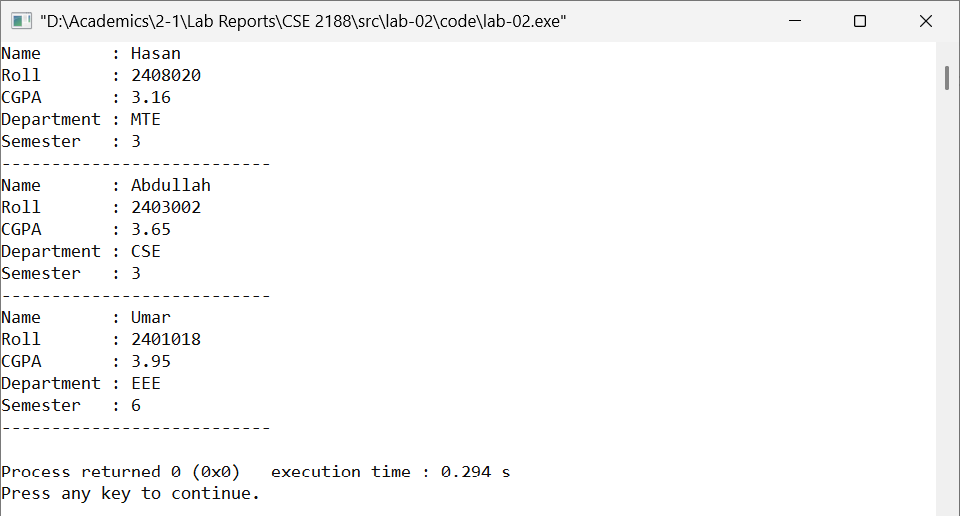
\includegraphics[width=0.8\textwidth]{lab-02/assets/output-student.png}
  \caption{Output of the Student Class Program.}
\end{figure}

\subsection{Problem 2: Book Class with Constructor and Destructor}
This program demonstrates the functionality of constructors and destructors in a C++ class. A \texttt{Book} class is created, where the constructor announces the creation of a book object and the destructor announces its removal.

\subsubsection{Code}
\begin{lstlisting}[language=C++, numbers=left]
#include <iostream>
using namespace std;

class Book {
    string title;
    string author;
    float price;

public:
    Book(string t, string a, float p) {
        title = t;
        author = a;
        price = p;
        cout << title << " added to library." << endl;
    }

    void display() {
        cout << "\nTitle  : " << title << endl;
        cout << "Author : " << author << endl;
        cout << "Price  : " << price << endl;
    }

    ~Book() {
        cout << title << " removed from library." << endl;
    }
};

int main() {
    Book b1("C++ Basics", "Bjarne", 450);
    Book b2("Data Structures", "Mark", 550);
    Book b3("Algorithms", "Thomas", 600);

    b1.display();
    b2.display();
    b3.display();

    return 0;
}

\end{lstlisting}

\subsubsection{Output}
\begin{figure}[H]
  \centering
  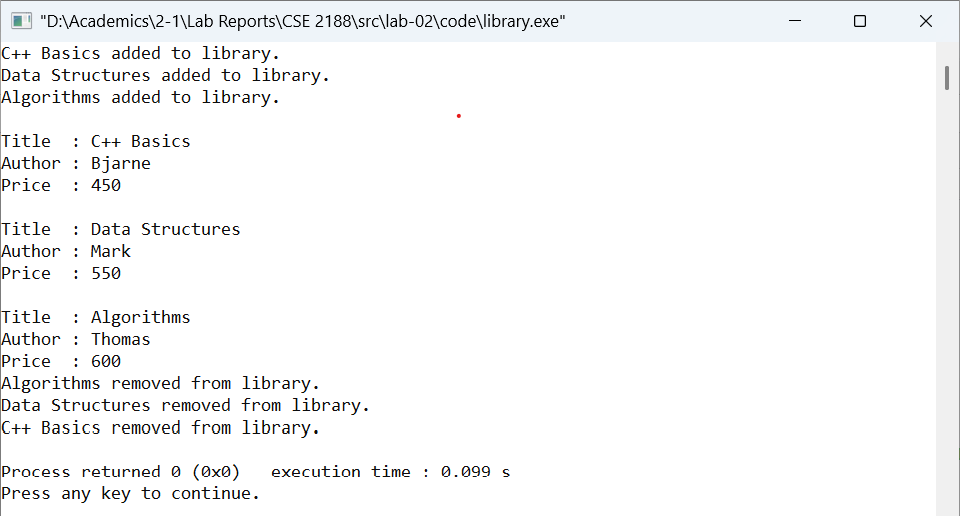
\includegraphics[width=0.8\textwidth]{lab-02/assets/output-library.png}
  \caption{Output of the Book Class Program.}
\end{figure}

\subsection{Problem 3: Motor Class for Electrical Calculations}
This program defines a \texttt{Motor} class to perform basic electrical calculations. It includes methods to calculate power, resistance, and energy, showcasing how classes can encapsulate data and related functionality.

\subsubsection{Code}
\begin{lstlisting}[language=C++, numbers=left]
#include <iostream>
using namespace std;

class Motor {
private:
    double voltage;
    double current;

public:
    // Constructor
    Motor(double v, double c) {
        voltage = v;
        current = c;
        cout << "Motor object created.\n";
    }

    double power() {
        return voltage * current;
    }

    double resistance() {
        if (current == 0) {
            cout << "Resistance cannot be calculated (Current = 0)." << endl;
            return 0;
        }
        return voltage / current;
    }

    double energy(double hours) {
        return power() * hours;
    }

    // Destructor
    ~Motor() {
        cout << "Motor object destroyed." << endl;
    }
};

int main() {
    Motor m1(24, 2.5);

    cout << "Power      : " << m1.power() << " W" << endl;
    cout << "Resistance : " << m1.resistance() << " Ohm" << endl;
    cout << "Energy (5h): " << m1.energy(5) << " Wh" << endl;

    return 0;
}

\end{lstlisting}

\subsubsection{Output}
\begin{figure}[H]
  \centering
  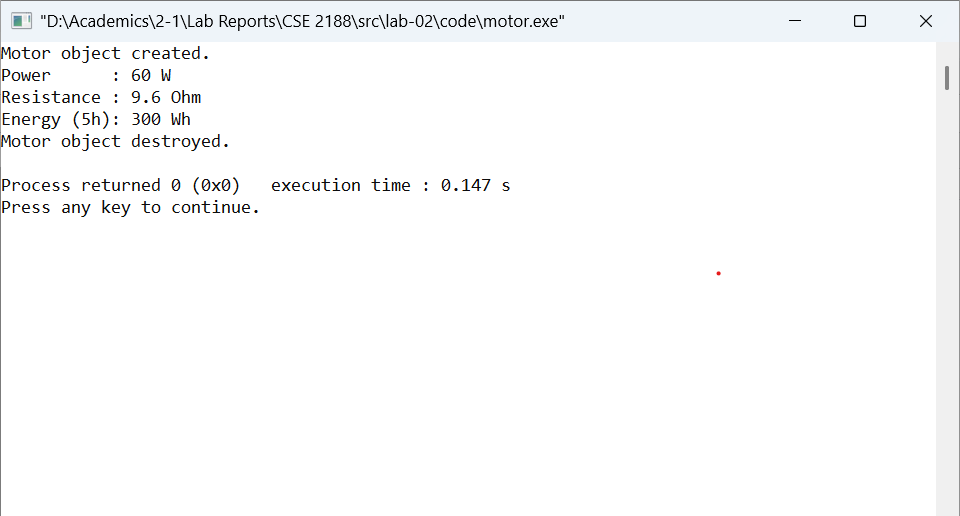
\includegraphics[width=0.8\textwidth]{lab-02/assets/output-motor.png}
  \caption{Output of the Motor Class Program.}
\end{figure}
